\documentclass[a4paper,11pt]{article}

% Add style file.
\usepackage{explanation}

% TMP...
\usepackage{lipsum}

% Add bib file for literature.
\addbibresource{explanation.bib}

\title{Implementing Deep Visual Odometry\\{\large Final Task of the course \emph{Implementing ANNs with Tensorflow}}}
\author{Rasmus Diederichsen \and Christian Heiden \and Alexander Mock\\\and \href{mailto:rdiederichse@uos.de}{rdiederichse@uos.de}\and \href{mailto:cheiden@uos.de}{cheiden@uos.de} \and \href{mailto:amock@uos.de}{amock@uos.de}}

\begin{document}

% Title
\maketitle


% --------------------- %
% SECTION: INTRODUCTION %
% --------------------- %
\section{Introduction}
\label{sec:introduction}
% TODO: Explain how visual odometry is useful
% TODO: Explain the structure of this paper
In robotics, the localization of a robot within its environment is an essential task. Especially in the days of autonomously driving vehicles this field of research receives a significant amount of attention. There are many ways to perform robot localization and usually several methods are used at the same time in order to improve reliability of the whole system. The main task of a localization algorithm is to repeatedly estimate the current pose of the robot. A pose is a 6-\emph{d} vector containing the $x$, $y$, $z$ positional values, as well as the \emph{yaw}, \emph{pitch}, and \emph{roll} values representing the rotation of the robot.

One approach of relative localization is \emph{odometry}. In most applications
odometry denotes the usage of wheel or motor movement data for estimating the
change in position over time (similar method to the speed estimation in a car).
Other sensors such as interial measurement units (IMUs) can also be fused with
odometry data. This method only provides relative localization which in this case means that the starting point of the robot is used as a reference position. In other words all estimated poses are in a coordinate system which is initially defined by the starting pose. Figure~\ref{fig:reference_frame} depicts a graphical explanation of the localization algorithm where the arrows show the change of the position over time.

\begin{figure}[tbh]
    \centering
    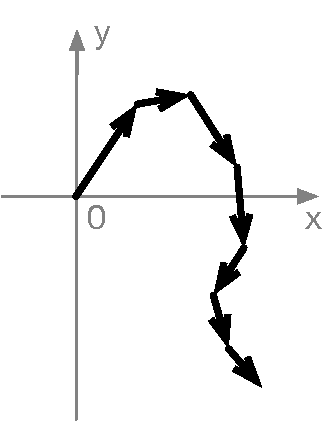
\includegraphics[width=0.2\linewidth]{reference_frame.pdf}
    \caption{Graphical explanation of the estimated positions of the robot over time. The starting position defines the center of the reference coordinate system.}
    \label{fig:reference_frame}
\end{figure}

Another relative localization approach is \emph{visual} odometry which tries to
fulfill the same goal as simple odometry but instead of motor or wheel
movements, it uses camera images. Classic approaches use techniques like optical
flow or feature matching between successive images in order to determine a
direction of movement between those two points in time.

The method we are going to present in this work is a visual odometry-based
approach but uses deep learning for determining the change of movement between
successive images. The original paper by Wang \etal{} \cite{wang2017deepvo} was
published in 2017 and describes the structure of a deep neural network
and evaluates its performance on the well-known KITTI dataset
which contains camera images and pose estimations of a car (a detailed
explanation is given in section~\ref{sec:deepvo:original}.

This paper is structured as follows. Section~\ref{sec:deepvo:original} presents
the idea and structure of the DeepVO Network and
Section~\ref{sec:deepvo:approach} gives a short explanation of how we
implemented it in TensorFlow. Section~\ref{sec:evaluation:data} will elaborate
on how we gathered data for training and testing. In
Section~\ref{sec:evaluation:results} we present the training behavior and
performance results of the our DeepVO implementation.


% --------------- %
% SECTION: DeepVO %
% --------------- %
\section{DeepVO Model}
\label{sec:deepvo}
In this section, the DeepVO network is presented (see Section~\ref{sec:deepvo:original}) together with our variant implemented in TensorFlow (see Section~\ref{sec:deepvo:approach}).


% -------------------------- %
% SUBSECTION: ORIGINAL PAPER %
% -------------------------- %
\subsection{Original Paper}
\label{sec:deepvo:original}

\begin{figure}[tbh]
    \centering
    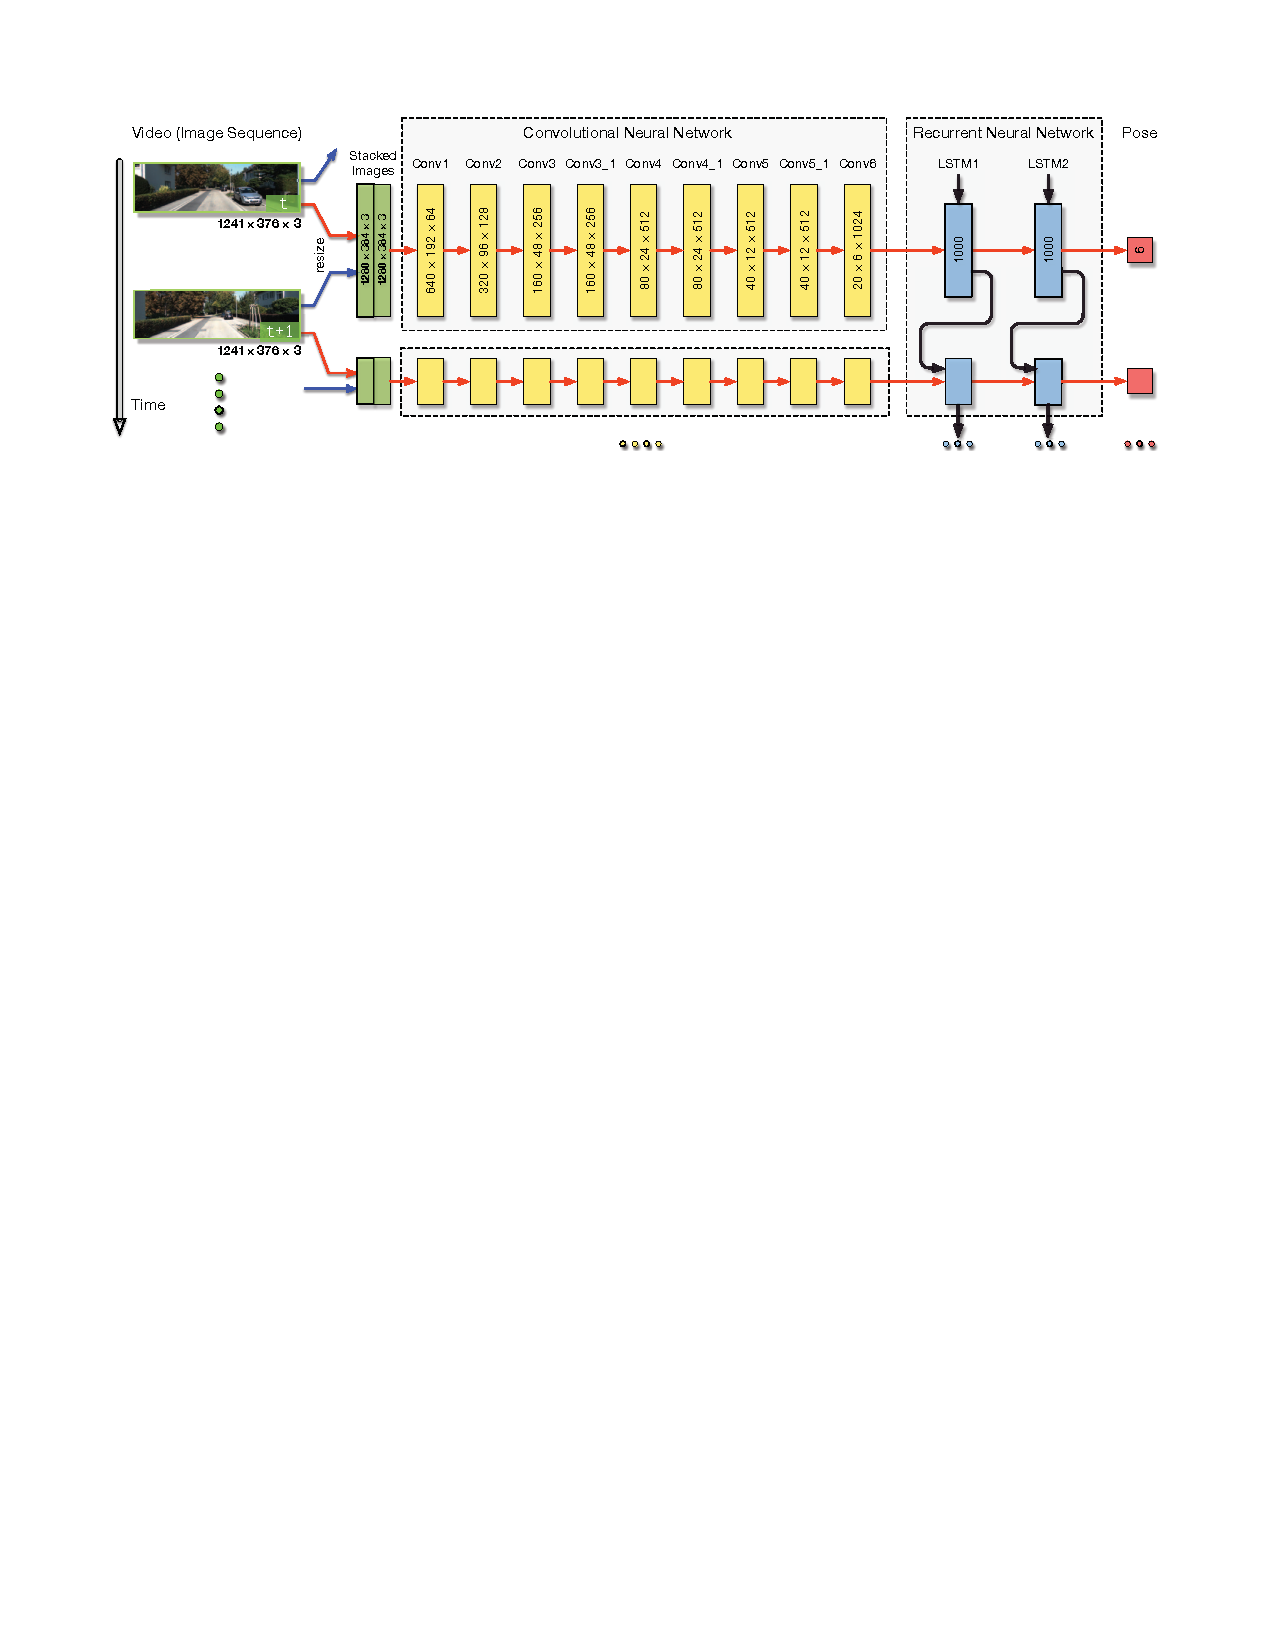
\includegraphics[width=\linewidth]{network.pdf}
    \caption{The structure of the network. Figure taken from \cite{wang2017deepvo}.}
    \label{fig:network}
\end{figure}

% TODO: Explain the deepVO model

The architecture for end-to-end learning of robot pose estimation is a recurrent
CNN where the convolutional portion is based on FlowNetSimple \citep{flownet} to
estimate the optical flow between successive images. \autoref{fig:architecture}
shows the network. Two successive images are stacked together and labeled with
the second image's pose


% -------------------- %
% SUBSECTION: APPROACH %
% -------------------- %
\subsection{Our Approach}
\label{sec:deepvo:approach}
% TODO: Explain how we implemented the model described in the paper
% TODO: --> This includes other implementations we found on the web? or problems we had, or simply stuff we did'nt know better


% ------------------- %
% SECTION: EVALUATION %
% ------------------- %
\section{Evaluation}
\label{sec:evaluation}
In this Section the data acquisition for training and testing is presented (see Section~\ref{sec:evaluation:data}), as well as the training progress and its performance results (see Section~\ref{sec:evaluation:results}).


% --------------------------- %
% SUBSECTION: DATA ACQUISTION %
% --------------------------- %
\subsection{Data Acquisition}
\label{sec:evaluation:data}
\begin{figure}[htb]
    \centering
    \begin{subfigure}[t]{0.6\linewidth}
            \centering
            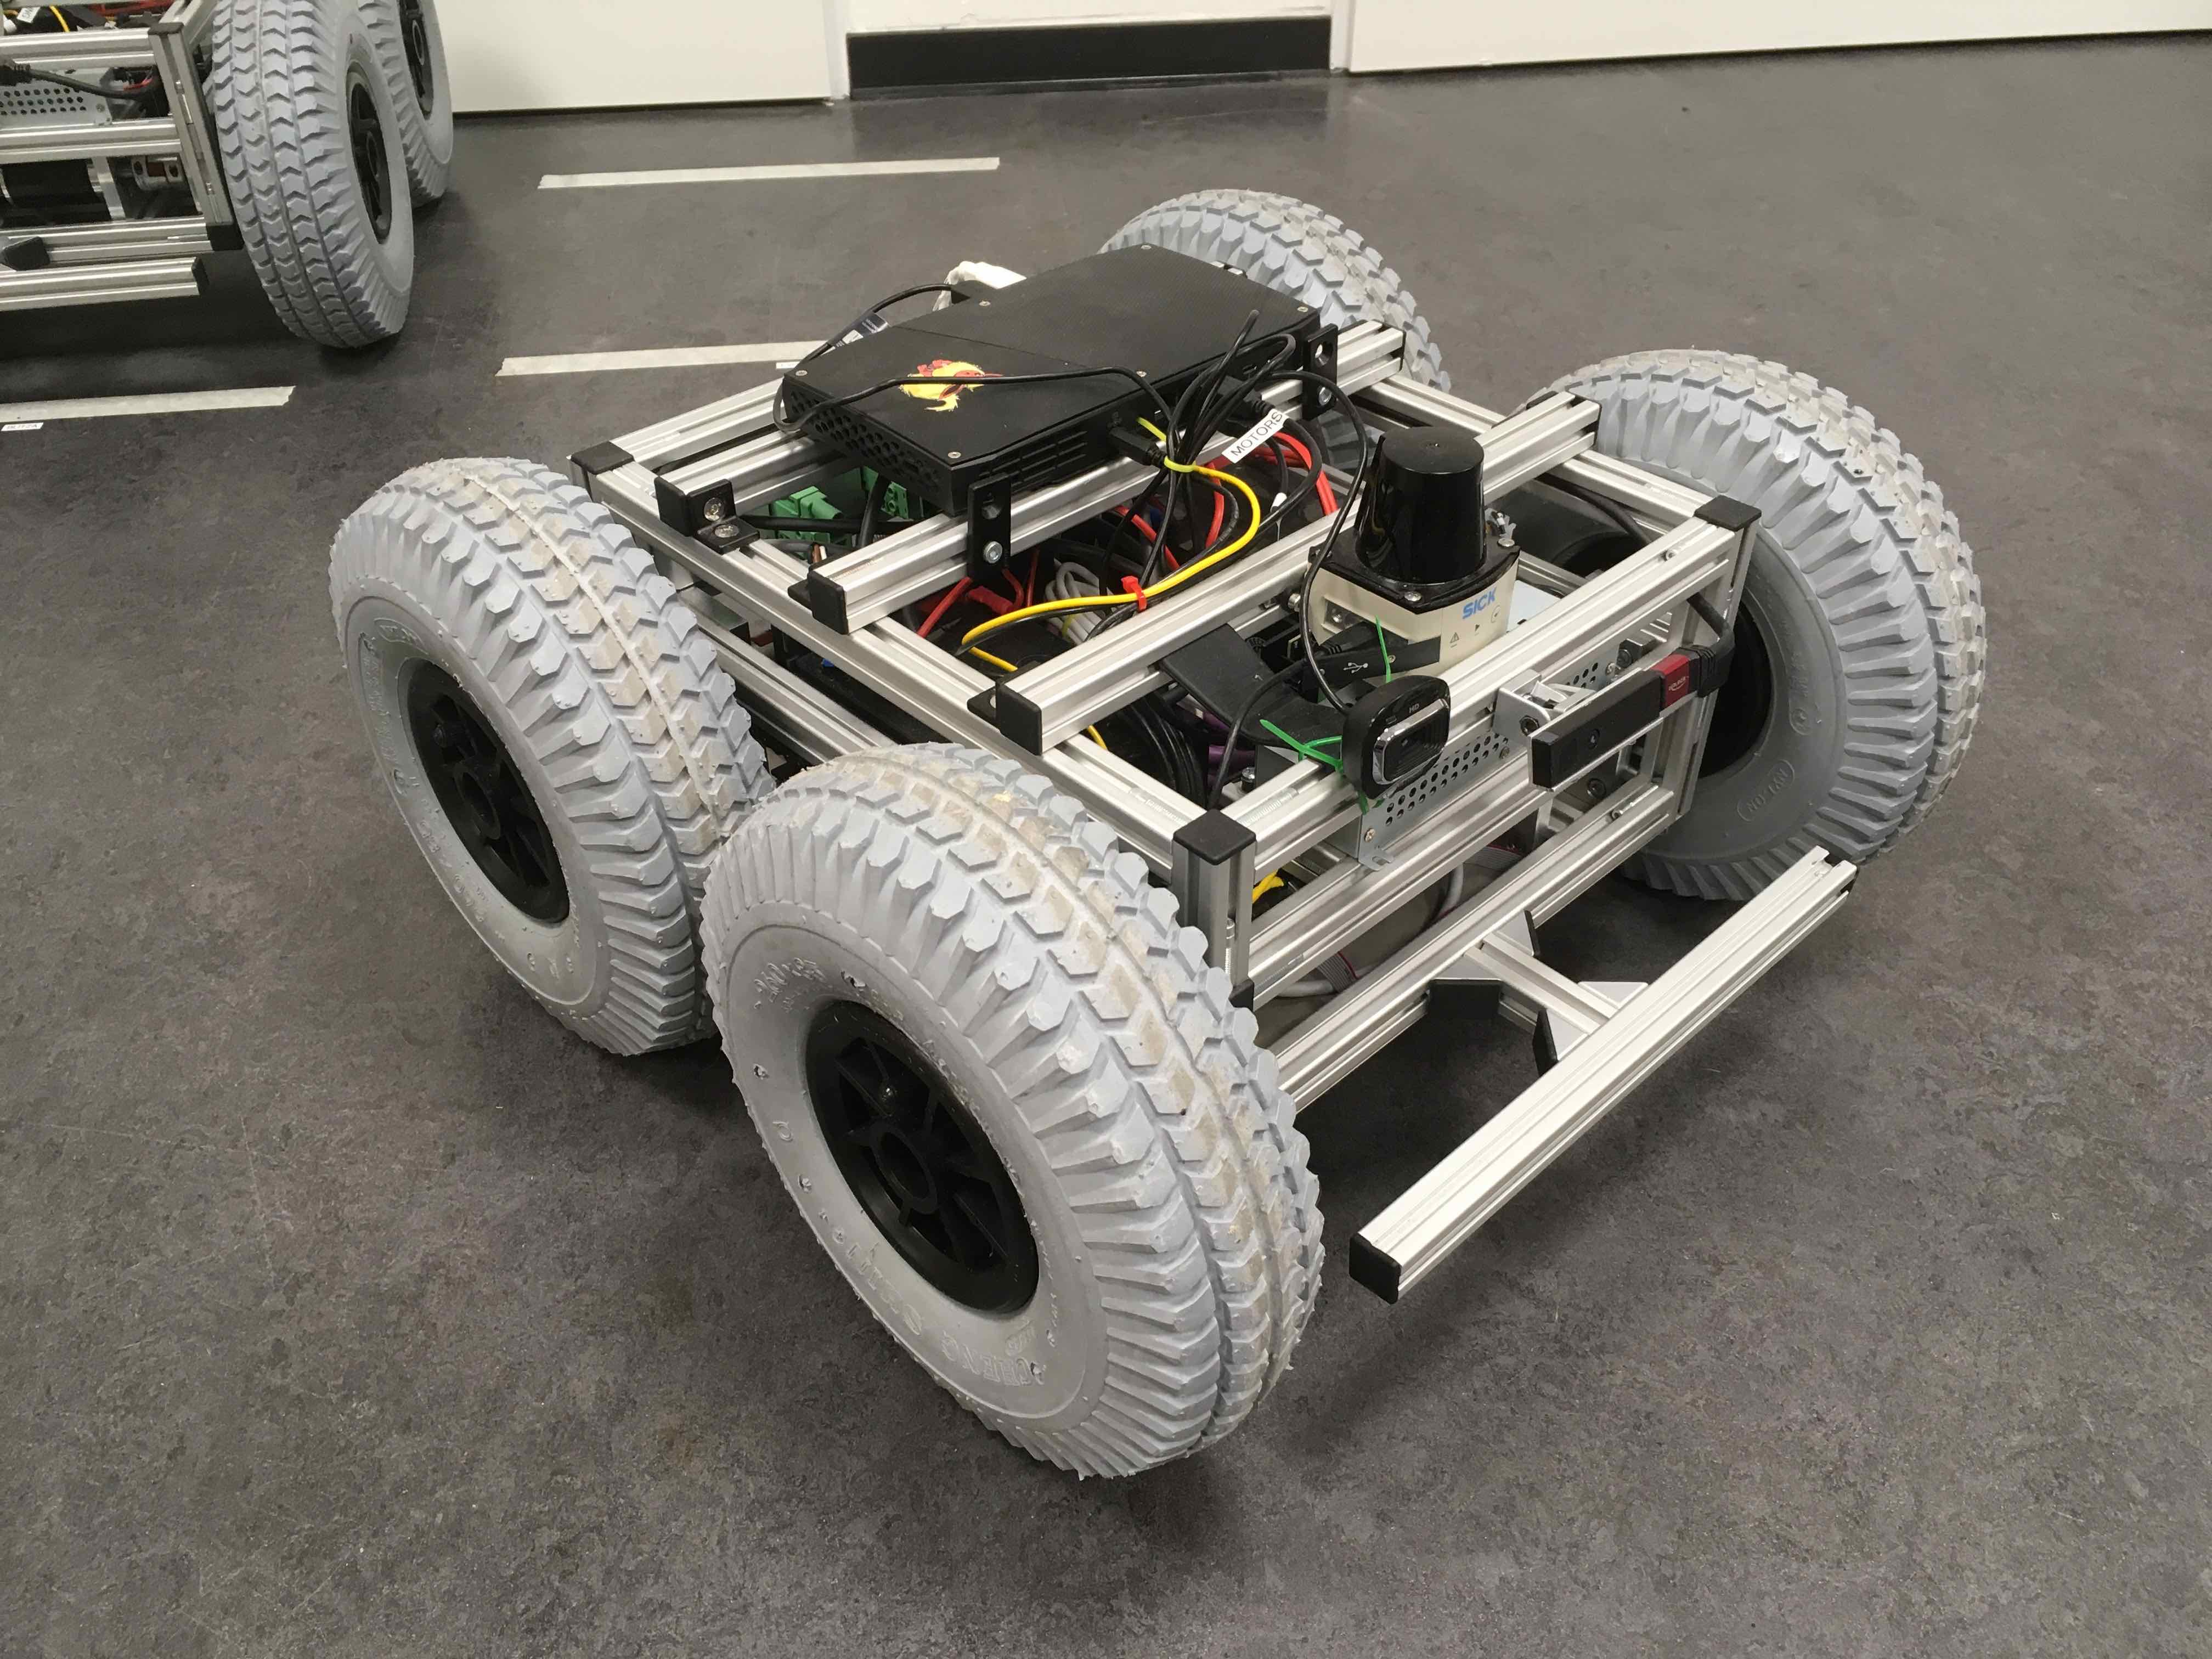
\includegraphics[width=0.9\linewidth]{robot_small.jpg}
            \caption[]{The ceres robot used for data acquisition.}
            \label{fig:robot}
    \end{subfigure}
    \begin{subfigure}[t]{0.39\linewidth}
            \centering
            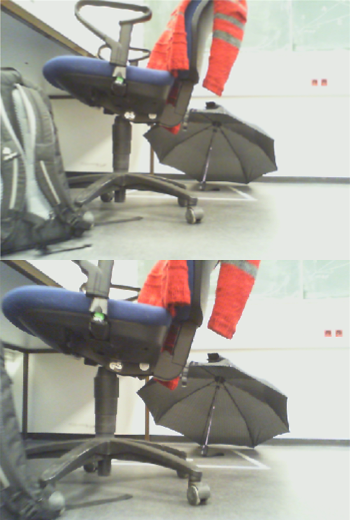
\includegraphics[width=0.75\linewidth]{image_pair.png}
            \caption[]{Exemplary successive images taken from the robots camera.}
            \label{fig:camera_images}
    \end{subfigure}
    \caption[]{Both figures depict the setup of our data acquisition.}
    \label{fig:setup}
\end{figure}

% TODO: 
% - Das ist der Roboter
% - Eigene Daten aufnehmen
%   - ROSbags mit Images und poses
%       - ApproximateTimeSynchronizer
% 
% - preprocessing
%   - float/mean images
% 
% - Data Handling
%   - Sequences 
%       - relative poses
%       - stacked images
%   - Shuffling
%   - test & training data batches


% ------------------- %
% SUBSECTION: RESULTS %
% ------------------- %
\subsection{Results}
\label{sec:evaluation:results}
% TODO: Show the results
Tba.

% ---------------------- %
% SUBSECTION: GREETINGS %
% ---------------------- %
\section{Room for Nonsense}
\label{sec:nonsense}
% TODO: Whatever is missing put it in here?!


% --------------------- %
% SECTION: BIBLIOGRAPHY %
% --------------------- %
\newpage
\printbibliography


\end{document}
